\chapter{How to Speak}

This lecture treats speaking as a practical craft with real stakes. It begins with a severe motivational claim, compresses that claim into a small formula for communicative quality, and then unfolds the formula into a repertoire of heuristics, room choices, media choices, props, slide law, job-talk structure, memorable framing, and endings. The order matters. We are first told why speaking matters, then how attention fails, then how a speaker can deliberately build structures that keep an audience with us.

\section{Opening Hook, Formula, and Promise}

The lecture opens with an analogy meant to be a little shocking. One does not send a soldier into battle without a weapon, and one ought not send students into life without the ability to communicate. The point is not ornament. The point is leverage. Winston states the ranking bluntly:

\begin{equation}
\text{speaking} \succ \text{writing} \succ \text{quality of ideas}.
\end{equation}

Here the symbol \(\succ\) is only editorial shorthand for his phrase ``in that order.'' The claim is worldly rather than metaphysical: it is about what determines whether ideas are heard, valued, and accepted.

That claim is then narrowed into a compact formula. In cleaned form, and following the secure transcript lines rather than the partially visible later blackboard residue, we may write

\begin{equation}
Q = f(K,P,T),
\end{equation}

where \(Q\) is the quality of communication, \(K\) is knowledge, \(P\) is practice, and \(T\) is inherent talent.

The asymmetry in the formula matters more than the formula itself. Winston immediately tells us that the \(T\) is very small. In a compact mathematical shorthand, not his own board notation but faithful to his meaning, one could summarize the point as

\begin{equation}
T \ll K,P.
\end{equation}

The lecture does not leave this as abstraction. It tests the formula with the Mary Lou Retton skiing anecdote. The contrast is sharp: Retton is an extraordinary athlete, but she is a novice skier; Winston is a far less gifted athlete, but a better skier. On this task, the relevant \(K\) and \(P\) outweigh raw \(T\). That is the first argument of the lecture: communicative excellence is not reserved for the naturally gifted.

\subsection{Question \& Answer}

\paragraph{Question.} Why is \(T\) small?

\paragraph{Answer.} Because talent detached from task-specific knowledge and repeated practice does not yet yield performance. The skiing story is the lecture's first proof-by-example. Retton brings enormous athletic talent, but Winston has the skiing knowledge and skiing practice. Therefore he skis better. The same structure is meant to transfer to speaking. A person with modest native gifts but good models, practiced habits, and disciplined preparation can outrun a more talented but less prepared speaker.

From here the lecture turns promise into motive. We are told that the next hour will offer an armamentarium of speaking techniques, and that perhaps one of them, maybe only one, will turn out to be the one that gets a person the job. This too is a mathematical way of thinking, though not as an equation: the process is nonlinear. Not every useful idea contributes equally. One local improvement may change an outcome disproportionately.

\section{Rules of Engagement and How to Start}

Before advice on speaking, Winston imposes a rule of engagement: no laptops, no cellphones. This is not presented as etiquette. It is presented as cognitive mechanics. We are told that human beings have one language processor. If that processor is occupied by reading email or browsing the web, then it is not available for listening. Worse, the distraction propagates outward: nearby listeners are disrupted, and the speaker also performs worse when he sees open laptops.

This claim returns later in the lecture, especially in the critique of text-heavy slides. Its role here is to clear the ground. Speaking is not merely the production of words; it is the management of a shared channel of attention.

The same argument then governs the beginning of a talk. Winston rejects the common advice to open with a joke. The reason is temporal. At the beginning, the audience is still settling, still adjusting to the speaker's vocal parameters, still arriving cognitively. The joke therefore lands before the audience is ready to receive it.

\subsection{Question \& Answer}

\paragraph{Question.} Why not start with a joke?

\paragraph{Answer.} Because the beginning of a talk is an adjustment phase, not yet a payoff phase. The audience has not synchronized with the speaker's timing, tone, or diction. A joke depends on precisely that synchronization. What belongs at the beginning instead is an empowerment promise: a statement of what the audience will know, understand, or be able to do by the end that they do not possess at the beginning.

This is one of the lecture's self-referential strengths. Winston is already doing what he recommends. He has opened with urgency, then a formula, then an anecdotal proof, and then a promise: by the end of the hour, the audience will possess a repertoire of usable speaking techniques.

\section{The Four Heuristics}

Having established that speaking contains knowledge, Winston next offers four sample heuristics that are ``always on my mind'' when he speaks: cycle on the subject, build a fence around the idea, use verbal punctuation, and ask a question.

\paragraph{Cycle.} The first heuristic is to go around the subject, and then go around it again. Winston glosses this with the old advice: tell them what you are going to tell them, tell them, and then tell them again. The lecture's justification is not contempt for the audience's intelligence. It is a model of intermittent attention: at any given moment, some part of the room is fogged out.

A useful editorial gloss can make the logic visible. If we denote by \(p_{\mathrm{fog}}\) the probability that a listener is mentally off the bus at a given pass, Winston's \(20\%\) heuristic gives

\begin{align}
p_{\mathrm{fog}} &\approx 0.2,\\
\mathrm{Prob}(\text{miss all three passes}) &\approx p_{\mathrm{fog}}^3 = 0.2^3 = 0.008,\\
\mathrm{Prob}(\text{catch at least one pass}) &\approx 1-p_{\mathrm{fog}}^3 = 0.992.
\end{align}

\begin{remark}
This calculation is an editorial model, not one Winston performs on the blackboard. Its value is explanatory. The lecture's actual point is that repeated passes give an audience multiple re-entry points.
\end{remark}

\subsection{Question \& Answer}

\paragraph{Question.} Why say it three times?

\paragraph{Answer.} Because speaking unfolds in time, and listeners drift in and out. A single pass is fragile. A second and third pass, especially if they are not perfectly identical but approach the same point from slightly different angles, dramatically increases the chance that the room catches the idea. ``Cycle'' is therefore not redundancy for its own sake. It is a technique for robustness.

\paragraph{Build a fence.} The second heuristic is to separate our idea from nearby but non-identical ideas. Winston's simple example is the arch: this is an arch; this is not an arch; that is not an arch. The more technical version is equally important: my algorithm may look like Jones's algorithm, except his is exponential and mine is linear. A definition becomes more useful when it is bounded by near misses and contrast cases.

\paragraph{Verbal punctuation.} The third heuristic exists for the same reason. If listeners fog out, they need seams at which they can get back in. Enumeration, recap, and explicit transitions create those seams. ``First,'' ``second,'' ``now the third idea,'' and ``next thing on our agenda'' are not filler phrases. They are re-entry markers.

\paragraph{Ask a question.} The fourth heuristic is to pose a question to the room. This is another way to bring listeners back onto the bus. It interrupts passive listening and forces orientation toward a problem.

Winston supplies a practical timing rule:

\begin{equation}
t_{\mathrm{wait}} \approx 7\,\mathrm{s}.
\end{equation}

Seven seconds feels very long to the speaker. That is exactly why it matters. The audience needs time to think, and a speaker who panics too early destroys the question. At the same time, the question must be chosen well: not so obvious that answering it feels embarrassing, and not so hard that silence is guaranteed.

\section{Time and Place as Part of the Argument}

The lecture now widens from local speaking heuristics to environmental conditions. What is the best time for a lecture? Winston's answer is \(11\) a.m. The logic is practical: the audience is awake, not immediately after a meal, and not yet collapsing into fatigue. In the same spirit, a room should be well lit, because dim light is an invitation to sleep. It should be cased in advance, meaning inspected beforehand so that odd features are not discovered live. And it should be reasonably populated. A half-empty hall generates a bad social signal before the talk even begins.

The middle of the lecture survives visually in a blackboard layout that is itself part of the argument. The board is not just a place to write content. It is a spatial organizer of the talk.

\begin{figure}[h]
\centering

\includegraphics[width=0.95\textwidth]{lecture_11_figure_03.png}
\end{figure}

The value of the board here is not algebraic. It is architectural. On the left is a list of heuristic samples; on the right is a second block for time and place. The loop beside ``Cycle'' gives a small drawn image to the repeated-pass idea. This is exactly the sort of graphic assistance Winston is praising when he argues for blackboards.

A cleaned reconstruction of the layout is useful, especially because the right-hand checklist is only partly legible in the screenshot and must be completed from the transcript:

\begin{figure}[h]
\centering
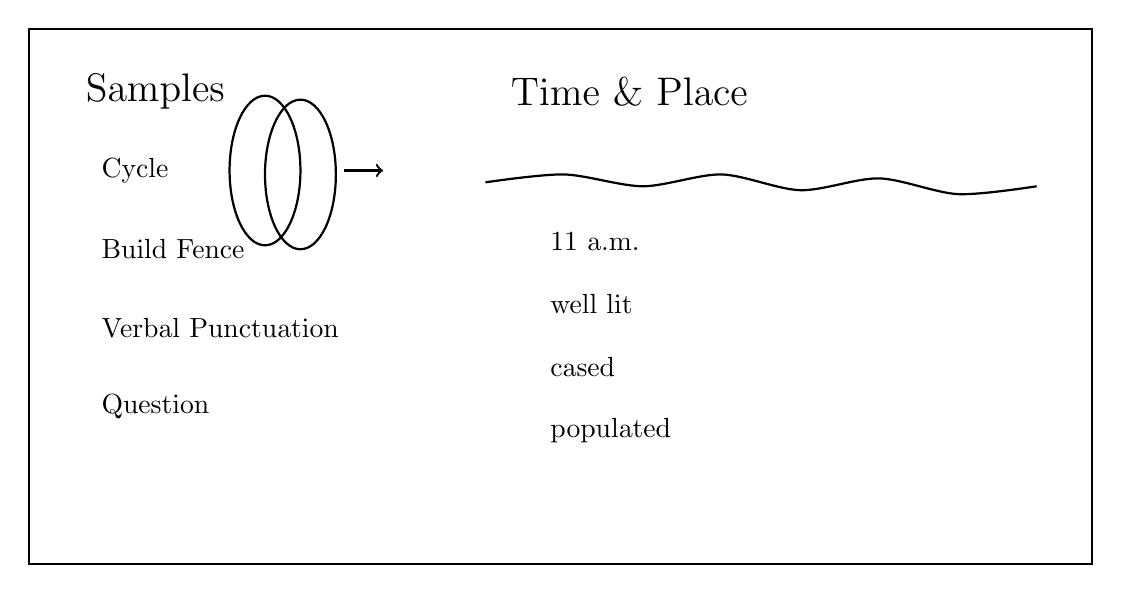
\begin{tikzpicture}[x=1cm,y=1cm]
\draw[thick] (0,0) rectangle (13.5,6.8);

\node[anchor=west] at (0.6,6.0) {\Large Samples};
\node[anchor=west] at (0.8,5.0) {Cycle};
\draw[thick] (3.0,5.0) ellipse (0.45 and 0.95);
\draw[thick] (3.45,4.95) ellipse (0.45 and 0.95);
\draw[->,thick] (4.0,5.0) -- (4.5,5.0);

\node[anchor=west] at (0.8,4.0) {Build Fence};
\node[anchor=west] at (0.8,3.0) {Verbal Punctuation};
\node[anchor=west] at (0.8,2.0) {Question};

\node[anchor=west] at (6.0,6.0) {\Large Time \& Place};
\draw[thick] plot[smooth] coordinates {(5.8,4.85) (6.8,4.95) (7.8,4.8) (8.8,4.95) (9.8,4.75) (10.8,4.9) (11.8,4.7) (12.8,4.8)};
\node[anchor=west] at (6.5,4.1) {11 a.m.};
\node[anchor=west] at (6.5,3.3) {well lit};
\node[anchor=west] at (6.5,2.5) {cased};
\node[anchor=west] at (6.5,1.7) {populated};
\end{tikzpicture}
\end{figure}

The lecture's point is that time and place are not peripheral logistics. They are upstream variables in the management of attention.

\section{Boards and Props}

Winston next compares boards, props, and slides. The contrast begins with purpose. Boards are the right tool when the aim is informing, teaching, or lecturing. Slides belong more naturally to exposing ideas, as in conference talks and job talks.

Three arguments are given for the board. First, it has graphic quality: it allows spatial grouping, headings, and quick sketches. Second, it has the correct speed property: the speed of writing on the board is roughly the speed at which an audience can absorb ideas. A slide deck can move much faster than comprehension. Third, the board gives the speaker's hands a target. This is a surprisingly physical point. Novice speakers suddenly become painfully aware of their hands; the board gives those hands something to do.

From there the lecture moves to props. The argument again comes by example rather than theory. Ibsen's pot-bellied stove in \emph{Hedda Gabler} builds tension because the object persists, gathers charge, and eventually seems destined to consume the manuscript. The point is memorable not because it is abstractly explained, but because the prop carries dramatic inevitability.

The same logic is then transferred to the classroom. Seymour Papert's bicycle wheel is not just a prop; it is a reasoning device.

\begin{figure}[h]
\centering

\includegraphics[width=0.78\textwidth]{lecture_11_figure_04.png}
\end{figure}

\subsection{Question \& Answer}

\paragraph{Question.} Which way does the spinning wheel go?

\paragraph{Answer.} Winston's answer is not to trust memorized hand rules. He says, in effect, that this leaves many otherwise well-trained people at about a \(50\%\) success rate, which is to say at the level of a coin toss. The better method is local rather than global.

\begin{enumerate}
\item Start the bicycle wheel spinning and imagine a small rim segment marked by duct tape.
\item Ignore the rest of the wheel for the moment.
\item Let the marked segment come over the top.
\item Apply the puff of air, or equivalently the local push, to that one segment.
\item Ask what that local piece now wants to do.
\item Observe that the next segment arriving at the top is in the same geometric situation.
\item Repeat the same local reasoning segment by segment.
\item Conclude that the whole wheel must roll in the corresponding direction.
\end{enumerate}

What matters pedagogically is the change of viewpoint. This is not presented as a gyroscopic derivation. It is a lesson in how to look at a problem so that the correct answer becomes almost forced.

The second prop example is the pendulum ball used to dramatize conservation of energy. A ball is pulled to nose height, released from rest, swings away, and returns to kiss but not crush the nose. The governing physics is canonical:

\begin{equation}
E = K_{\mathrm{kin}} + V_{\mathrm{pot}} = \text{const.}
\end{equation}

Again the mathematics is simple, but the memory of the demonstration is not. The real warning is not against energy conservation but against human overconfidence: the first-time demonstrator may push instead of merely letting go.

Only after the stove, the wheel, and the pendulum does Winston offer his general theory. Chalk and props work, he suggests, because of a kind of empathetic mirroring. When we watch a hand write on a board, or a ball swing in a room, we can almost feel ourselves doing it. Slides and pictures are missing that physical co-presence. Example first, explanation second: the order is important.

\section{Slides, Special Cases, and the Job Talk Threshold}

The lecture now turns sharply toward slides. Winston's basic distinction is clean: slides are for exposing ideas, not for teaching them. That already tells us what kinds of talk they suit.

The critique begins with a universal law: people almost always have too many slides and too many words. The crimes then follow in sequence. Do not read the slide to the audience; they know how to read already. Do not stand far from the slide and induce a visual tennis match between speaker and screen. Do not bury the main point in background junk, logos, titles that the speaker is already saying aloud, or bullet clutter.

The earlier one-language-processor claim now returns with force. When a slide is dense with text, audience members read instead of listening. Winston reinforces this with an experimental anecdote: when half the information is spoken and half displayed on the slide, students remember the slide material better. In the after-action report, one subject remarks that the speaker's talking was distracting. The remark is funny, but the principle is exact.

A practical typographic rule follows:

\begin{equation}
40\text{--}50\,\mathrm{pt}\ \text{is generally safe}, \qquad 35\,\mathrm{pt}\ \text{is already too small.}
\end{equation}

The point is not merely legibility in a narrow sense. Smaller fonts usually signal that the speaker is trying to force too much language onto the slide.

From here the lecture broadens again into special cases. To inform well, one should still begin with a promise, but inspiration requires more: telling people they can do it, helping them see a problem in a new way, and exhibiting genuine passion about the material. Winston's resource-allocation example makes the structure explicit. We are first shown an absurdly slow brute-force process and then promised that within the next fifty minutes a slight adjustment will transform geological time into seconds. The promise is simultaneously epistemic and emotional.

Oral exams bring two further principles into focus: situate the work in context and practice under realistic conditions. A student fails, Winston says, by speaking as though the work floated free of its field, or by rehearsing only in front of people who already know the content and therefore hallucinate missing explanations into the talk.

\subsection{Question \& Answer}

\paragraph{Question.} How long do you have in a job talk?

\paragraph{Answer.} Roughly five minutes.

\begin{equation}
t_{\mathrm{job}} \approx 5\,\mathrm{min}.
\end{equation}

Within that window, two things must already be established: first, that the speaker has vision; second, that the speaker has done something. ``Vision'' means a problem worth caring about together with a distinctive approach. ``Done something'' means more than vague aspiration. Winston recommends enumerating the steps required to solve the problem, showing which of those steps have actually been completed, and then mirroring those steps at the end in a contributions slide.

A compact technical-talk structure emerges:

\begin{enumerate}
\item State the important problem.
\item Show what is new in the approach.
\item Enumerate the steps needed for progress.
\item Demonstrate that some of those steps have in fact been carried out.
\item End by listing the contributions, which mirror the steps.
\end{enumerate}

That is already more than presentation advice. It is a theory of how a research talk becomes legible to strangers.

\section{Getting Remembered and Knowing How to Stop}

Once the job is obtained, Winston says, the next question is not celebrity in the shallow sense but recognition in the serious sense. The line he offers is memorable: one never gets used to being ignored. Packaging is therefore not vanity; it is a way of ensuring that ideas do not go out into the world in rags.

The memory device he proposes is Winston's Star, a five-part structure:

\begin{itemize}
\item symbol,
\item slogan,
\item surprise,
\item salient idea,
\item story.
\end{itemize}

The old arch-learning example lets him unpack the star. The arch itself is the symbol. ``One-shot learning'' is the slogan. The surprise is that one does not need a million examples; one good example can teach something definite. The salient idea is not generic importance but the thing that sticks out, here the notion of a near miss. And all of it must be embedded in a story of how the system works and why the result matters.

The lecture then turns to endings. This is another place where Winston proceeds by staging failures first. One should not end with an enormous collaborator list, because that dilutes agency at precisely the moment when the audience is trying to remember what the speaker has done. One should not end with a wasted blank slide, nor with a generic ``conclusions'' slide that leaves the wrong abstraction in the audience's head.

\subsection{Question \& Answer}

\paragraph{Question.} What should the final slide and final words do?

\paragraph{Answer.} The final slide should display contributions, and the final words should perform a genuine closing gesture rather than merely signal politeness.

The last slide remains on the screen while questions are asked and while people are filing out. It should therefore keep the audience looking at the strongest compression of what has been achieved. ``Contributions'' is the right label because it mirrors the earlier enumeration of what had to be done.

The final words are a separate matter. Winston allows that a joke can work at the end, because by then the audience has adjusted to the speaker and can receive the timing properly. What he resists is ending with ``thank you'' as the main final act. That phrase suggests that the audience has endured the talk out of politeness and is now being thanked for its endurance. Better endings perform closure more positively: a benediction, a formal dismissal, or a salute to the audience and the place.

The lecture itself closes in that spirit. Winston tells the audience that by showing up they have already demonstrated an understanding that presentation matters, and he salutes them for it. Only after the real closing gesture does a final courtesy thank-you appear.

\section{Summary}

The lecture's argument can be read as a sequence of reductions. First, speaking is reduced from mystique to craft by the formula \(Q=f(K,P,T)\), with talent explicitly demoted. Next, craft is reduced to a repertoire of practical heuristics for coping with intermittent attention. Then those heuristics are embedded in room choice, board use, props, and slide discipline. Finally, the same logic is compressed again into job-talk thresholds, memory structures, and ending moves.

What holds the chapter together is a single problem: how do ideas survive contact with time, distraction, embodiment, and audience memory? Winston's answer is not a single technique. It is a layered method. We motivate, we promise, we cycle, we fence, we punctuate, we ask, we choose our tools well, and we close on the strongest possible reminder of what has been done.